\section{Derivation of ROC and PR curve baselines}
\subsection{ROC curve baseline}\label{subsec:roc-curve-baseline-derivation}
Given that accuracy
\begin{align}
    \text{acc} &= \pi \cdot\text{TPR} + (1 - \pi) (1 - \text{FPR}),
\end{align}
which can be rewritten to $\text{TPR}$ in terms of $\text{FPR}$,
\begin{align}
    \text{TPR} &= \frac{\text{acc}}{\pi} - \frac{(1-\pi)}{\pi}(1 - \text{FPR}) \\
               &= \frac{\text{acc}}{\pi} - \frac{(1-\pi)}{\pi} + \frac{1-\pi}{\pi}\text{FPR} \\ 
               &= \frac{\text{acc} - 1 + \pi}{\pi} + \frac{1-\pi}{\pi}\text{FPR}.
\end{align}
In the case of an always positive classifier that is right for $\pi$ of the time,
\begin{align}
    \text{TPR}(\text{acc} = \pi) = \frac{1-\pi}{\pi}\text{FPR} + 2 - \frac{1}{\pi}.
\end{align}

\subsection{PR curve baseline}\label{subsec:pr-curve-baseline-derivation}
Given that the $F_1$-score is
\begin{align}
    F_1 &= \frac{2}{\text{prec}^{-1} + \text{rec}^{-1}},
\end{align}
which can be rewritten as
\begin{align}\label{eq:prec-in-terms-of-rec}
    \text{prec} = \frac{F_1 \cdot \text{rec}}{2\cdot \text{rec} - F_1}.
\end{align}
The $F_1$-score of an always positive classifier is
\begin{align}
    F_{1, +} &= \frac{2 \cdot \text{prec}}{\text{prec} + 1},
\end{align}
since in this case $\text{prec} = \pi$ and $\text{rec} = 1$.
Substituting $F_1$ in \cref{eq:prec-in-terms-of-rec} for $F_{1, +}$, we get
\begin{align}
    \text{prec} = \frac{F_{1, +} \cdot \text{rec}}{2\cdot \text{rec} - F_{1, +}}.
\end{align}

\section{Flow of images to splits}\label{app:folds-splits-viz}
The splits are created as described in \cref{subsec:models}.
The process is visualized in \cref{fig:folds-splits-viz}.

\begin{figure*}
    \centering
    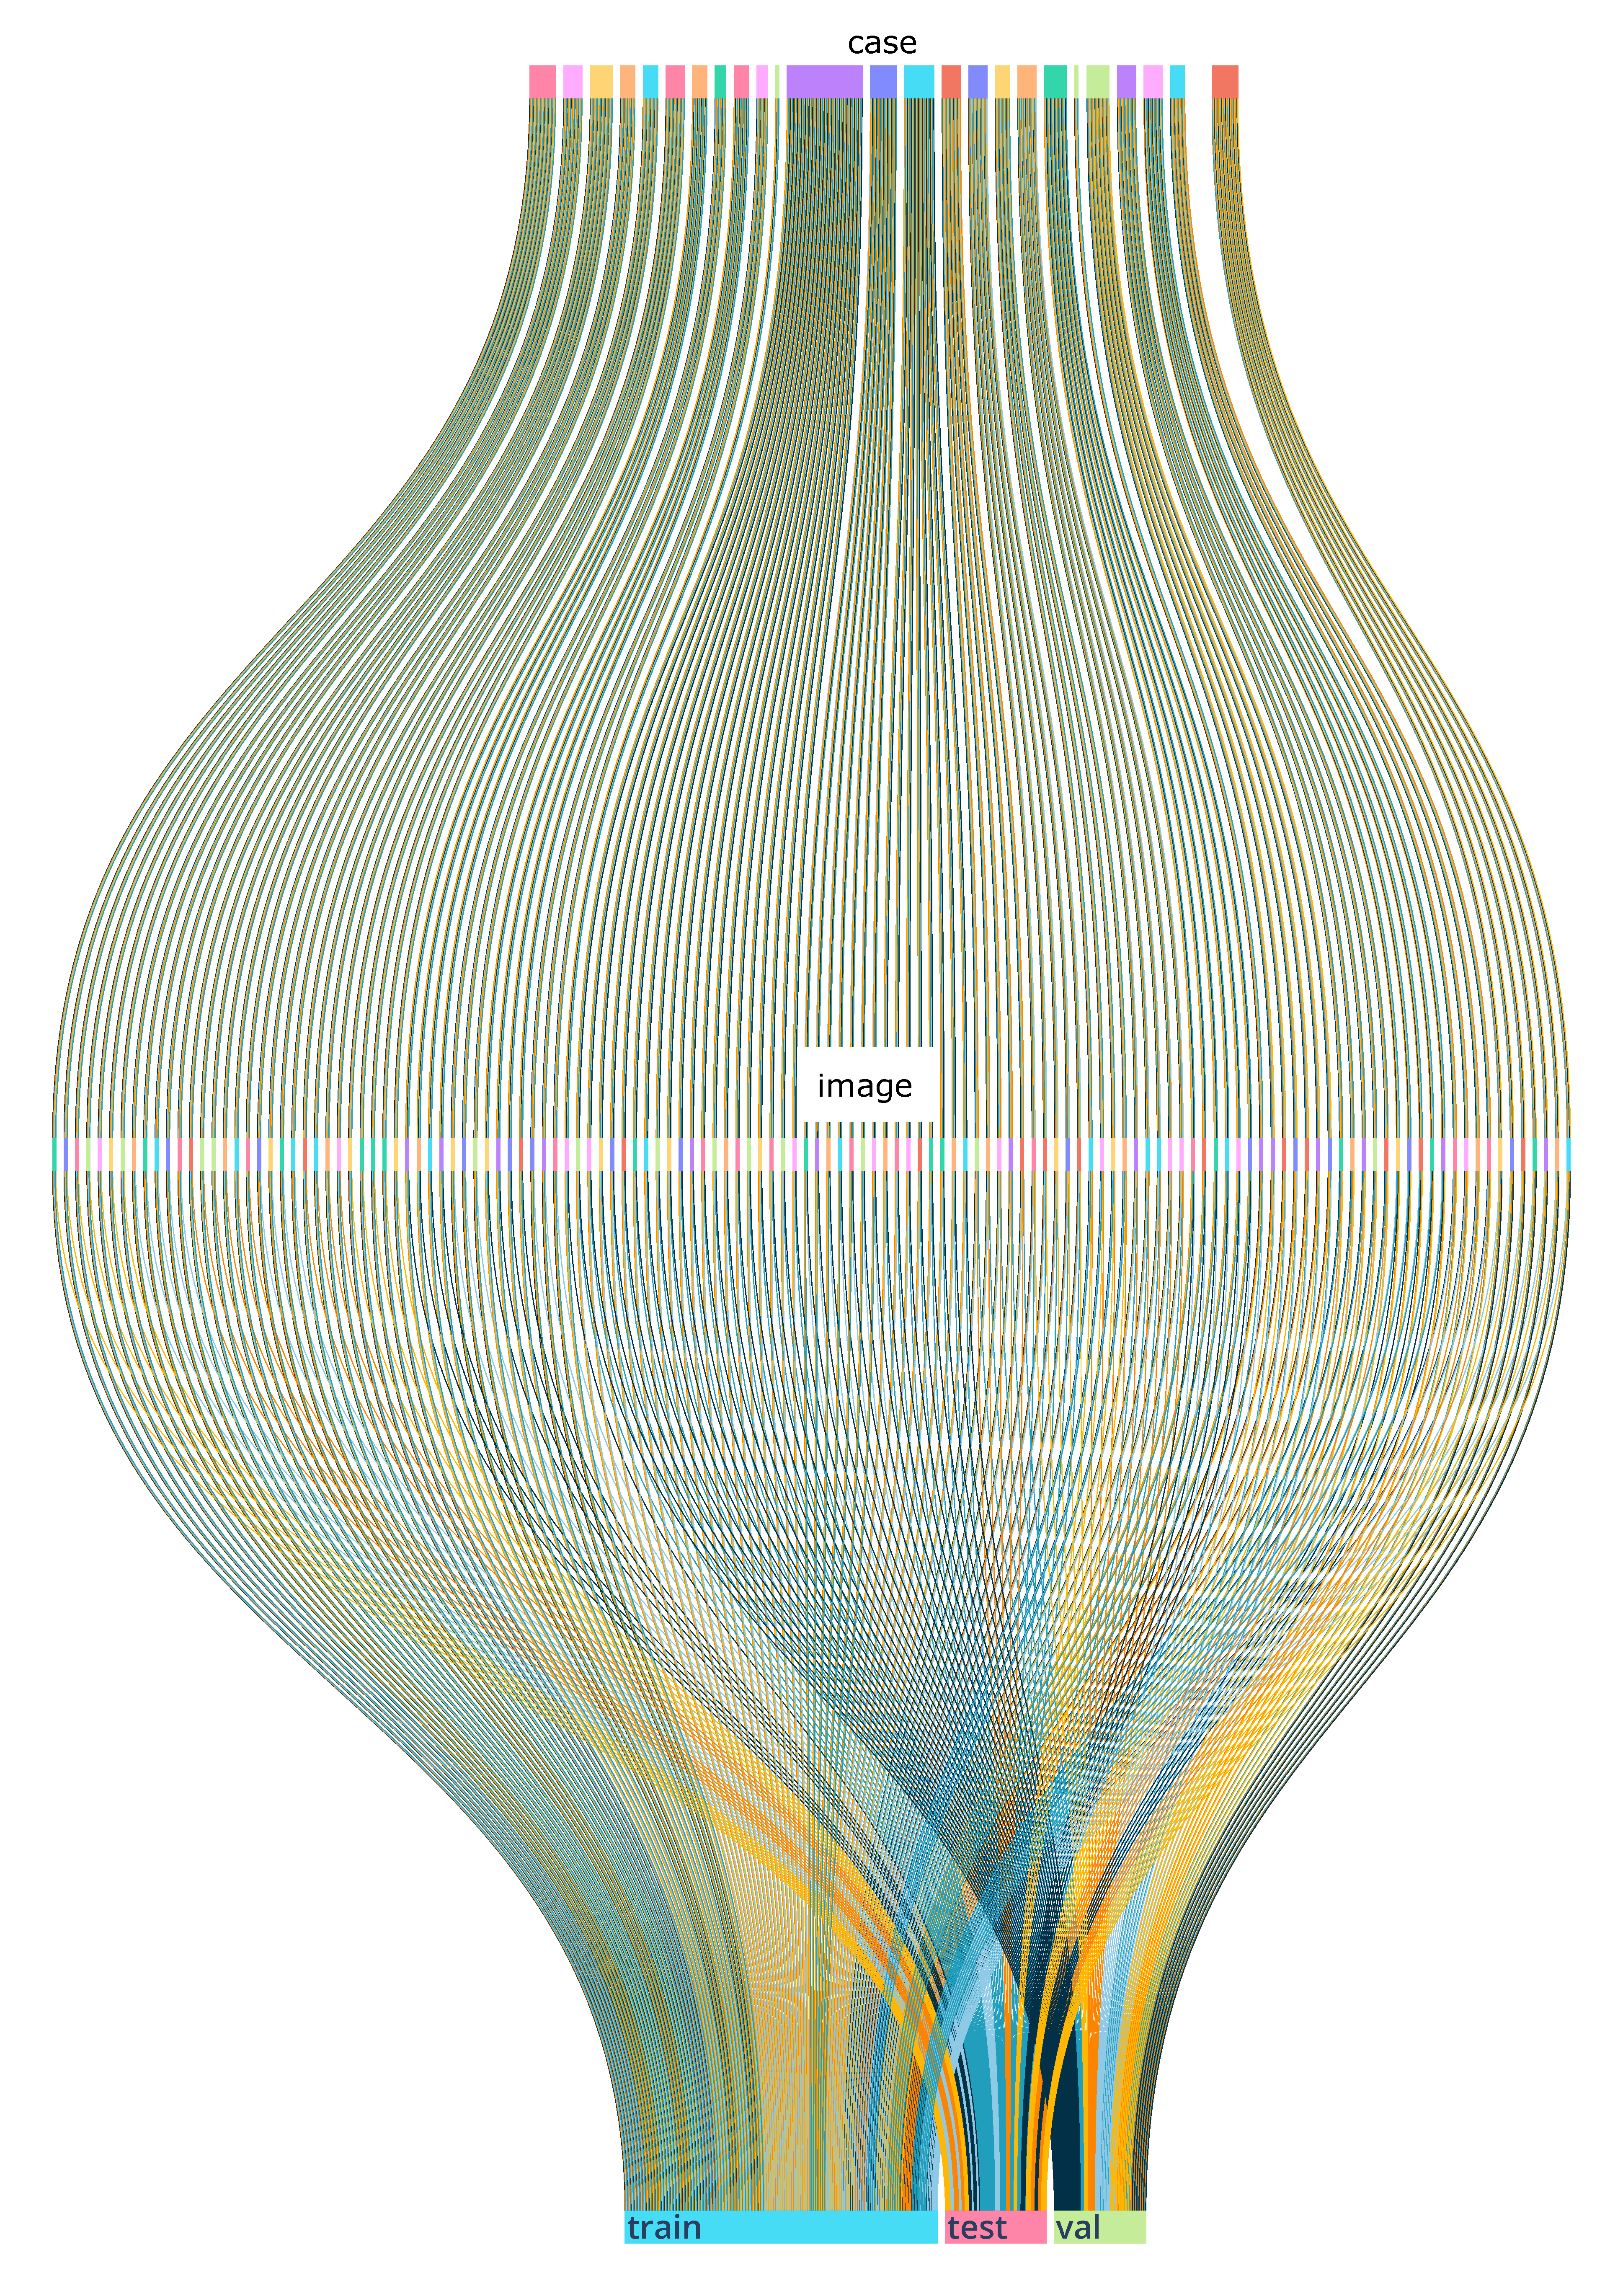
\includegraphics[height=0.55\paperheight]{pediatric-brain-tumours/images/folds-splits-viz.pdf}
    \caption[Flow of images to splits]{
        The flow of images to splits.
        Top row shows available cases.
        Every block is one case.
        Middle row shows available images and is linked to the cases.
        Bottom row shows training, validation and test splits.
        Colors show flow within one fold.
        Manual zoom may show details.
    }
    \label{fig:folds-splits-viz}
\end{figure*}

\section{Software diagrams}\label{app:sclicom_c4}
The first level of the C4 model sets the context of the software and is shown in \cref{fig:context_diagram}.
The second level shows the high-level technical building blocks of the software and is shown in \cref{fig:container_diagram}.

\begin{figure*}
    \centering
    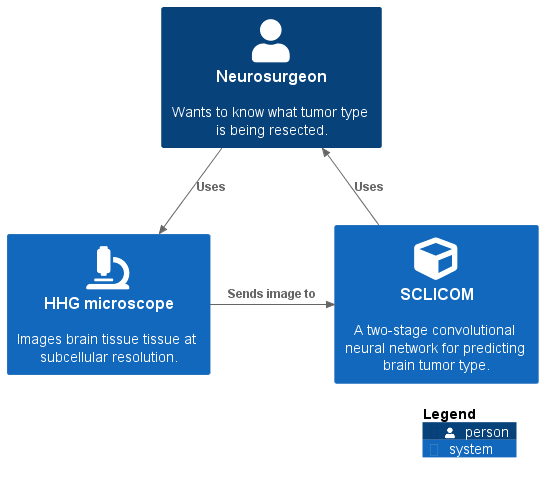
\includegraphics[width=\linewidth]{images/System_context_diagram.png}
    \caption[SCLICOM system context diagram]{
        System context diagram of SCLICOM.
        A neurosurgeon or technician images brain tumors using an HHG microscope.
        The microscope output serves as input to SCLICOM, a convolutional neural network to predict brain tumors imaged by the microscope.
        The trained model can help intraoperatively diagnose brain tumors, or provide specific regions to at for quicker diagnosis.
    }
    \label{fig:context_diagram}
\end{figure*}

%%% https://tex.stackexchange.com/questions/272486/fit-sidewaysfigure-to-page-width-including-caption-and-source
\begin{figure*}
    \centering
    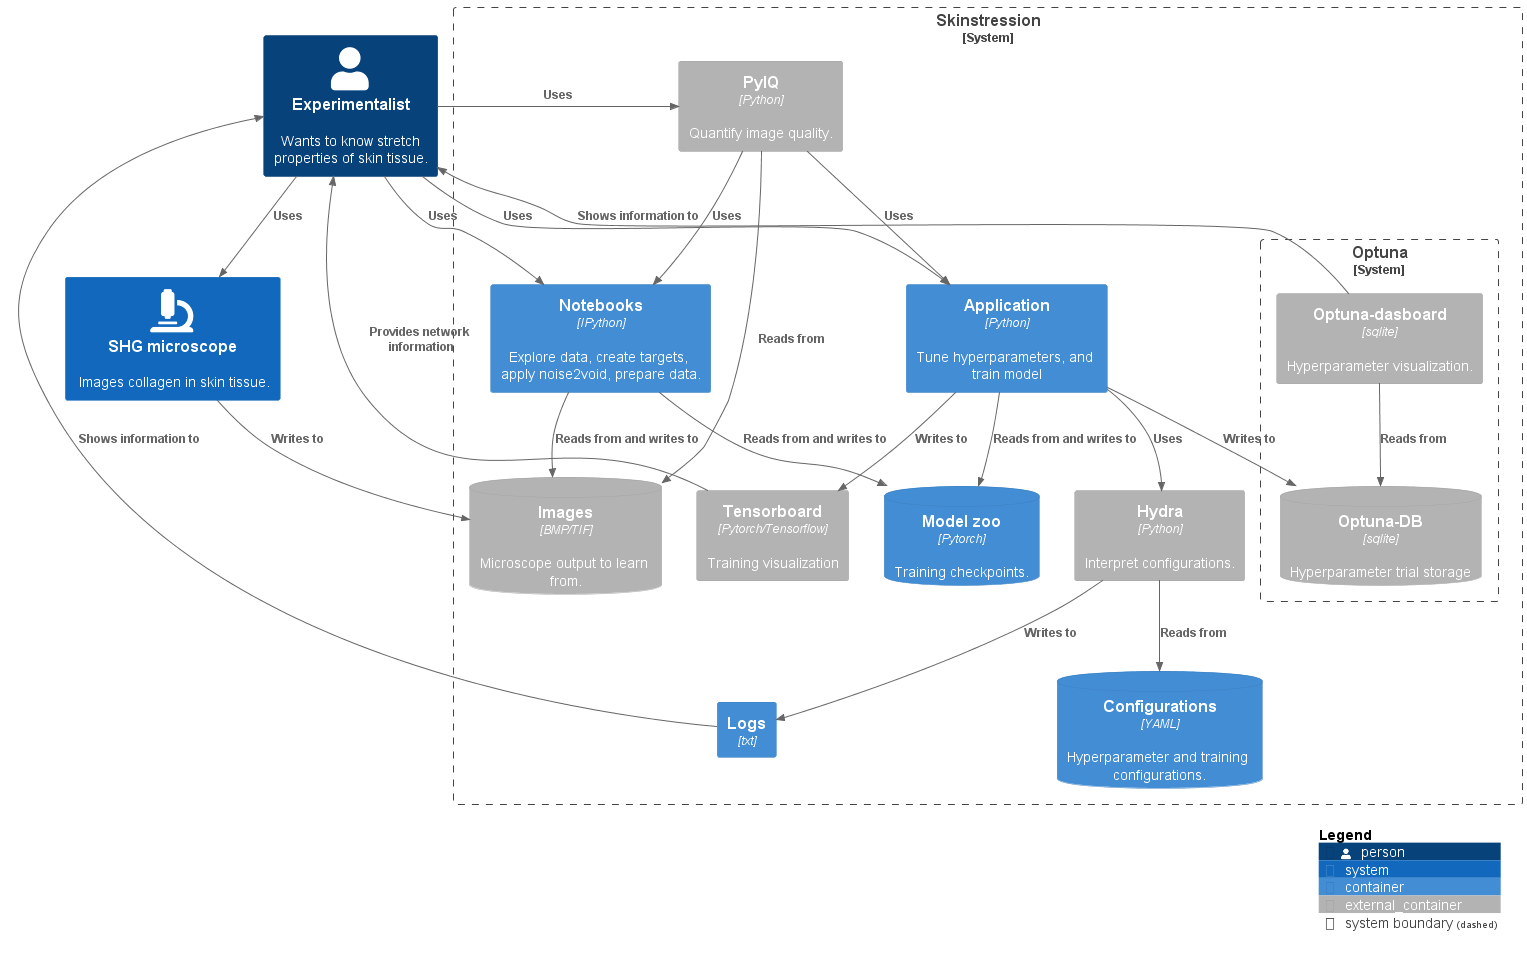
\includegraphics[angle=90, width=0.9\textheight,height=\linewidth,keepaspectratio]{images/Container-diagram.png}
    \caption[SCLICOM container diagram]{
        Container diagram of SCLICOM.
        The bounding box shows internal communications of SCLICOM.
        Images generated with the HHG microscope get stored.
        The main application reads locally stored configurations and trains with Pytorch Lightning.
        Trained models are stored in the model zoo.
        Hyperparameter optimizations and resources are tracked by Ray Tune.
        Training and hyperparameter optimization can be inspected by Tensorboard.
        The application logs output and errors to text files.
    }
    \label{fig:container_diagram}

\end{figure*}
